\section{Le langage GRAFCET}

Le langage GRAFCET, aussi appelé SFC (Sequentiel Function Chart) est, comme son nom l'indique, dédié à la description et à la programmation de \textbf{problèmes séquentiels}. Il décrit donc une suite d'étapes séparées par des transitions.

Un GRAFCET est très proche conceptuellement d'une machine à état. Il est représenté tel que sur la Figure~\ref{fig:simpleGrafcet}

\begin{figure}[ht]
  \centering
  \begin{tikzpicture}
\EtapeInit[0,0]{100}
\Transition[VX100]{100}
\Etape[VT100]{110}
\Transition{110}
\Etape[VT110]{120}
\Transition[VX120]{120}
\LienRetour{T120}{X100}
\Recept{T100}{$dcy \cdot a_0$}
\ActionX{X110}{Sortir Noyau}
\Recept{T110}{condition}\ActionX{X120}{Rentrer Noyau}
\Recept{T120}{$a_0$}
\end{tikzpicture}

  \caption{GRAFCET simple composé de trois étapes}
  \label{fig:simpleGrafcet}
\end{figure}

\subsection{Étapes et actions}

Une étape est représentée par un carré comportant un numéro (Figure~\ref{fig:etape}). Elle est généralement associée à une  (Figure~\ref{fig:etapeAction}) ou plusieurs (Figure~\ref{fig:etapeDeuxActions}) actions.
Il est également possible d'ajouter une condition à une action (Figure~\ref{fig:etapeActionCond}).

\UPSTIaRetenir{\begin{itemize}
  \item Une action associée à une étape n'est effectuée que lorsque cette étape est active.
  \item Une action conditionnelle est effectuée lorsque \textbf{l'étape est active et que la condition associée est vérifiée}.
\end{itemize}}

Il également possible d'effectuer une action qu'au moment de l'activation d'une étape (Figure~\ref{fig:etapeActivation}). Cela est particulièrement utile pour incrémenter un compteur.
En effet, sans cela l'action \textit{compteur = compteur + 1} serait effectuée durant toute la durée de l'action associée. Cela incrémenterait le compteur à chaque cycle automate donc approximativement toutes les \SI{10}{ms}.

Pour un grafcet en cours d'exécution, on peut représenter l'étape active dans un grafcet à l'aide d'une étoile comme illustré sur la Figure~\ref{fig:etapeActive}.

\begin{figure}[ht]
\centering
  \begin{subfigure}[b]{.49\textwidth}
    \centering
    \begin{tikzpicture}
      \Etape[0,0]{110}
    \end{tikzpicture}
    \caption{Représentation d'une étape en GRAFCET}
    \label{fig:etape}
  \end{subfigure}%
  %
  \begin{subfigure}[b]{.49\textwidth}
    \centering
  \begin{tikzpicture}
    \Etape[0,0]{110}
    \ActionX{X110}{Sortir Noyau}
  \end{tikzpicture}
  \caption{Une étape et l'action associée}
  \label{fig:etapeAction}
  \end{subfigure}%
  %

  \begin{subfigure}[b]{.48\textwidth}
    \centering
  \begin{tikzpicture}
    \Etape[0,0]{110}
    \ActionX{X110}{Sortir Noyau, Allumer voyant}
  \end{tikzpicture}
  \caption{Une étape et deux actions simultanées. Les deux actions sont actives tant que l'étape 110 est active.}
  \label{fig:etapeDeuxActions}
  \end{subfigure}\hfill
%
  \begin{subfigure}[b]{.48\textwidth}
    \centering
  \begin{tikzpicture}
    \Etape[0,0]{110}
    \ActionX{X110}{Sortir Noyau}
    \ActionCond{X110}{$\overline{\text{defaut}}$}
  \end{tikzpicture}
  \caption{Une étape avec action conditionnelle : L'action \textit{Sortir Noyau} ne sera exécutée que si \textit{defaut} est à 0.}
  \label{fig:etapeActionCond}
  \end{subfigure}%

  \begin{subfigure}[b]{.48\textwidth}
    \centering
  \begin{tikzpicture}
    \Etape[0,0]{130}
    \ActionX{X130}{compteur = compteur + 1;}
    \ActionActiv{X130}
  \end{tikzpicture}
  \caption{Une étape et une action sur activation. L'action n'est effectuée qu'au moment de l'activation de l'étape.}
  \label{fig:etapeActivation}
  \end{subfigure}%
  %
  \begin{subfigure}[b]{.48\textwidth}
    \centering
  \begin{tikzpicture}
    \Etape[0,0]{110}
    \ActionX{X110}{Sortir Noyau}
    %\ActionCond{X110}{$\overline{\text{defaut}}$}
    \LienActivation{X110}
  \end{tikzpicture}
  \caption{Etape courramment active}
  \label{fig:etapeActive}
  \end{subfigure}
  \caption{Etapes et action(s) associée(s)}%
  %
\end{figure}


\subsection{Transitions}
\subsubsection{Généralités}
Une transition est \textbf{toujours} placée entre deux actions. Ce sont les transitions qui décrivent la façon de passer d'une action à une autre.
Une transition est associée à une \textbf{réceptivité} (Voir Figure~\ref{fig:transition}).

\UPSTIaRetenir{Une transition sera franchie si et seulement si l'étape précédente est active ET la réceptivité associée est vérifiée.}

\begin{figure}[ht]
  \centering
  \begin{subfigure}[b]{.48\textwidth}
    \centering
      \begin{tikzpicture}
        \Transition[0,0]{110}
      \end{tikzpicture}
    \caption{Une transition}
    \label{fig:transition}
  \end{subfigure}
  \begin{subfigure}[b]{.48\textwidth}
    \centering
      \begin{tikzpicture}
        \Transition[0,0]{110}
        \Recept{T110}{$dcy \cdot a_0$}
      \end{tikzpicture}
    \caption{Une transition et sa réceptivité associée}
    \label{fig:transitionEtRecept}
  \end{subfigure}
  \caption{Transitions et Réceptivité}
  %\label{fig:transitionEtReceptivite}
\end{figure}
\subsubsection{Différents types de transition}
\begin{figure}
\centering
    \begin{subfigure}[b]{.4\textwidth}
      \centering
        \begin{tikzpicture}
          \Transition[0,0]{110}
          \Recept{T110}{$a + \overline{b}$}
        \end{tikzpicture}
        \vspace{-30pt}
      \caption{Une combinaison (OU,ET,etc.)}
      \label{fig:transitionCombi}
    \end{subfigure}
    \begin{subfigure}[b]{.4\textwidth}
      \centering
        \begin{tikzpicture}
          \Transition[0,0]{110}
          \Recept{T110}{$\uparrow a$}
        \end{tikzpicture}\vspace{-30pt}
      \caption{Front montant}
      \label{fig:transitionFrontMontant}
    \end{subfigure}
\vspace*{10pt}

    \begin{subfigure}[b]{.3\textwidth}
      \centering
        \begin{tikzpicture}
          \Transition[0,0]{110}
          \Recept{T110}{$1$}
        \end{tikzpicture}\vspace{-30pt}
      \caption{Toujours \textbf{vraie}}
      \label{fig:transitionVraie}
    \end{subfigure}
    \begin{subfigure}[b]{.3\textwidth}
      \centering
        \begin{tikzpicture}
          \Transition[0,0]{110}
          \Recept{T110}{$a > 2$}
        \end{tikzpicture}\vspace{-30pt}
      \caption{Comparaison}
      \label{fig:transitionComparaison}
    \end{subfigure}
    \begin{subfigure}[b]{.3\textwidth}
      \centering
        \begin{tikzpicture}
          \Transition[0,0]{110}
          \Recept{T110}{$T/X110/5s$}
        \end{tikzpicture}\vspace{-30pt}
      \caption{Temporisation}
      \label{fig:transitionFrontMontant}
    \end{subfigure}
  \caption{Différents types de transitions}
  \label{fig:TypesTransition}
\end{figure}
\subsection{Saut d'étapes et reprise de séquence}
Le saut d'étapes permet de sauter une ou plusieurs étapes lorsque les actions associées sont inutiles à réaliser, La reprise de séquence (ou boucle) permet de reprendre, une ou plusieurs fois, une séquence tant qu'une condition n'est pas obtenue.


\subsection{Divergences et Convergences}
\subsubsection{Divergence/Convergence en OU}
On dit qu'il y a Aiguillage ou \textbf{divergence en OU} lorsque le grafcet se décompose en deux ou plusieurs séquences selon un choix conditionnel. Après une divergence en OU on rencontre souvent une \textbf{convergence en OU}. On dit qu'il y a convergence en OU, lorsque deux ou plusieurs séquences du grafcet converge vers une seule séquence.

 Un exemple est donnée en Figure~\ref{fig:divOU}.

\UPSTIaRetenir{\begin{itemize}
  \item Une divergence en \textbf{OU} est \textbf{toujours} suivie d'une transition sur chacune de ses branches.
  \item Une convergence en \textbf{OU} est \textbf{toujours} précédée d'une transition sur chacune de ses branches.
  \item Les conditions d'une divergence doivent être exclusives.
\end{itemize}}

\begin{figure}[ht]
  \centering
  \begin{tikzpicture}
  \Etape[0,0]{1}
  \DivOU{X1}{-5/L1a,3/L1b,11/L1c}
  \SequenceTT[L1a]{1a}{11}
  \SequenceTT[L1b]{1b}{21,22,23}
  \SequenceTT[L1c]{1c}{31,32}
  \ConvOU[-3]{T23}{T32,T11}{L2}
  \Etape[L2]{2}
  \DecaleNoeudy[-3]{VX2}{VX2}
  \DecaleNoeudy[-3]{NoeudGraf}{NoeudGraf}
  \Actions{1/A1,11/A11,21/A11,22/A22,
  23/A23,31/A31,2/A2}
  \Recepts{1a/r1a,1b/r1b,1c/r1c,11/r11,
  21/r21,22/r22,23/r23,31/r31,32/r32}
\end{tikzpicture}

  \caption{Exemple de divergence en \textbf{OU}. Une seule des branches est parcourrue.}
  \label{fig:divOU}
\end{figure}


\subsubsection{Divergence en ET}
Au contraire de l'aiguillage, où ne peut se dérouler qu'une seule activité à la fois, on dit qu'on se trouve en présence d'un parallélisme structurel (\textbf{divergence en ET}), si plusieurs activités indépendantes pouvent se dérouler en parallèle. Un parallélisme structurel commence par une divergence en ET et termine par une convergence en ET. Celles-ci sont représentées par deux traits parallèles. Un exemple est donnée en Figure~\ref{fig:divET}.

\UPSTIremarque{La dernière étape d'une divergence en ET est souvent vide pour attendre les autres branches.}
\begin{figure}
  \centering
  \begin{tikzpicture}
  \Etape{3}
  \Transition{3}
  \DivET{T3}{-6/br1,7/br3,20/br2}
  \Graphe[Vbr1]{
  21/Remplir cuve/ cuver remplie
  }
  \Etape{24}
  \Etape[Vbr2]{31}
  \SequenceEE[Vbr3]{11,12}{13}
  \ConvET[-7]{X13}{X24,X31}{b40}
  \Transition[b40]{40}
  \Etape{41}
  \ActionRecept{
  11/Sortir tige verin/tige sortie,
  12/Rentrer tige verin/tige rentrée
  }
  \ActionX{X31}{Allumer voyant}
  \Recept{T3}{$marche$}
  \Recept{T40}{$\underline1$}
\end{tikzpicture}

  \caption{Exemple de divergence en \textbf{ET}. Les trois branches sont parcourrue simultanéement.}
  \label{fig:divET}
\end{figure}

\subsection{Rêgles de conception}
\UPSTIaRetenir{\begin{itemize}
  \item Les actions ne concernent que les \textbf{actionneurs} ou des variables internes.
  \item Les réceptivités ne concernent que les capteurs ou des variables internes
  \item Une étape est \textbf{toujours} suivie d'une transition
  \item Une transition est \textbf{toujours} suivie d'une étape.
  \end{itemize}}

\subsection{Deux niveaux de GRAFCET}
On peut écrire les grafcet d'un point de vue fonctionnel ou d'un point de vue opérationnel. Ces deux points de vue sont décrits ci-dessous et illustrés en Figure~\ref{fig:fonctionnelVsOperationnel}.
\subsubsection{Niveau fonctionnel (Fig~\ref{fig:grafcetFonct})}
Ce grafcet utilise des mots du cahier des charges. C'est la première étape d'élaboration d'un programme. Il est destiné à être compris par tous les collaborateurs d'un projet. Ce sont donc des verbes qui sont utilisés pour décrire les actions d'une étape.
\subsubsection{Niveau opérationnel~\ref{fig:operationnel}}
Ce niveau de grafcet sert à la programmation de l'automate. C'est celui qui sera retranscrit dans le logiciel de programmation et envoyé à l'automate. Il est souvent moins lisible que le grafcet fonctionnel et est destiné aux intervenants sur la partie opérative.

Ce grafcet est décrit à l'aide des noms de variables associées aux entrées (pour les réceptivités) et aux sorties (pour les actions) de l'automate.


\begin{figure}
  \centering
  \begin{subfigure}[b]{.48\textwidth}
    \input{grafcet_diagrams/fonctionnel.tikz}
    \caption{Fonctionnel}
    \label{fig:grafcetFonct}
  \end{subfigure}
  \begin{subfigure}[b]{.48\textwidth}
    \begin{tikzpicture}
\EtapeInit[0,0]{100}
\Transition[VX100]{100}
\Etape[VT100]{110}
\Transition{110}
\Etape[VT110]{120}
\Transition[VX120]{120}
\LienRetour{T120}{X100}
\Recept{T100}{$dcy$}
\ActionX{X110}{V+}
\Recept{T110}{fcV}
\ActionX{X120}{V-}
\Recept{T120}{$a_0$}
\end{tikzpicture}

    \caption{Opérationnel}
    \label{fig:operationnel}
  \end{subfigure}
  \caption{Grafcets fonctionnel et opérationnel}
  \label{fig:fonctionnelVsOperationnel}
\end{figure}
